\documentclass[11pt]{article}
\usepackage[textwidth=18.0cm, textheight=23.0cm, top=2.0cm]{geometry}
\usepackage{pst-all}
\usepackage{amssymb}
\usepackage{tikz}
\usepackage{underscore}\begin{document}
\pagestyle{empty}


ClassName: \underline{\textbf{Class_08.2bp-28}}
\par
BinSize: \underline{\textbf{100 × 100}}
\par
ReduceSize: \underline{\textbf{100 × 100}}
\par
TypeNum: \underline{\textbf{59}}
\par
Num: \underline{\textbf{60}}
\par
OutS: \underline{\textbf{170000}}
\par
InS: \underline{\textbf{136674}}
\par
Rate: \underline{\textbf{0.804}}
\par
UB: \underline{\textbf{17}}
\par
LB0: \underline{\textbf{17}}
\par
LB: \underline{\textbf{17}}
\par
LBWithCut: \underline{\textbf{17}}
\par
NodeCut: \underline{\textbf{0}}
\par
ExtendedNodeCnt: \underline{\textbf{1}}
\par
GenNodeCnt: \underline{\textbf{1}}
\par
PrimalNode: \underline{\textbf{0}}
\par
ColumnCount: \underline{\textbf{17}}
\par
TotalCutCount: \underline{\textbf{0}}
\par
RootCutCount: \underline{\textbf{0}}
\par
LPSolverCnt: \underline{\textbf{1}}
\par
PricingSolverCnt: \underline{\textbf{0}}
\par
BranchAndBoundNum: \underline{\textbf{1}}
\par
isOpt: \underline{\textbf{true}}
\par
TimeOnInitSolution: \underline{\textbf{600.000 s}}
\par
TimeOnPrimal: \underline{\textbf{0.000 s}}
\par
TimeOnPricing: \underline{\textbf{0.000 s}}
\par
TimeOnRmp: \underline{\textbf{0.063 s}}
\par
TotalTime: \underline{\textbf{600.328 s}}
\par
\newpage


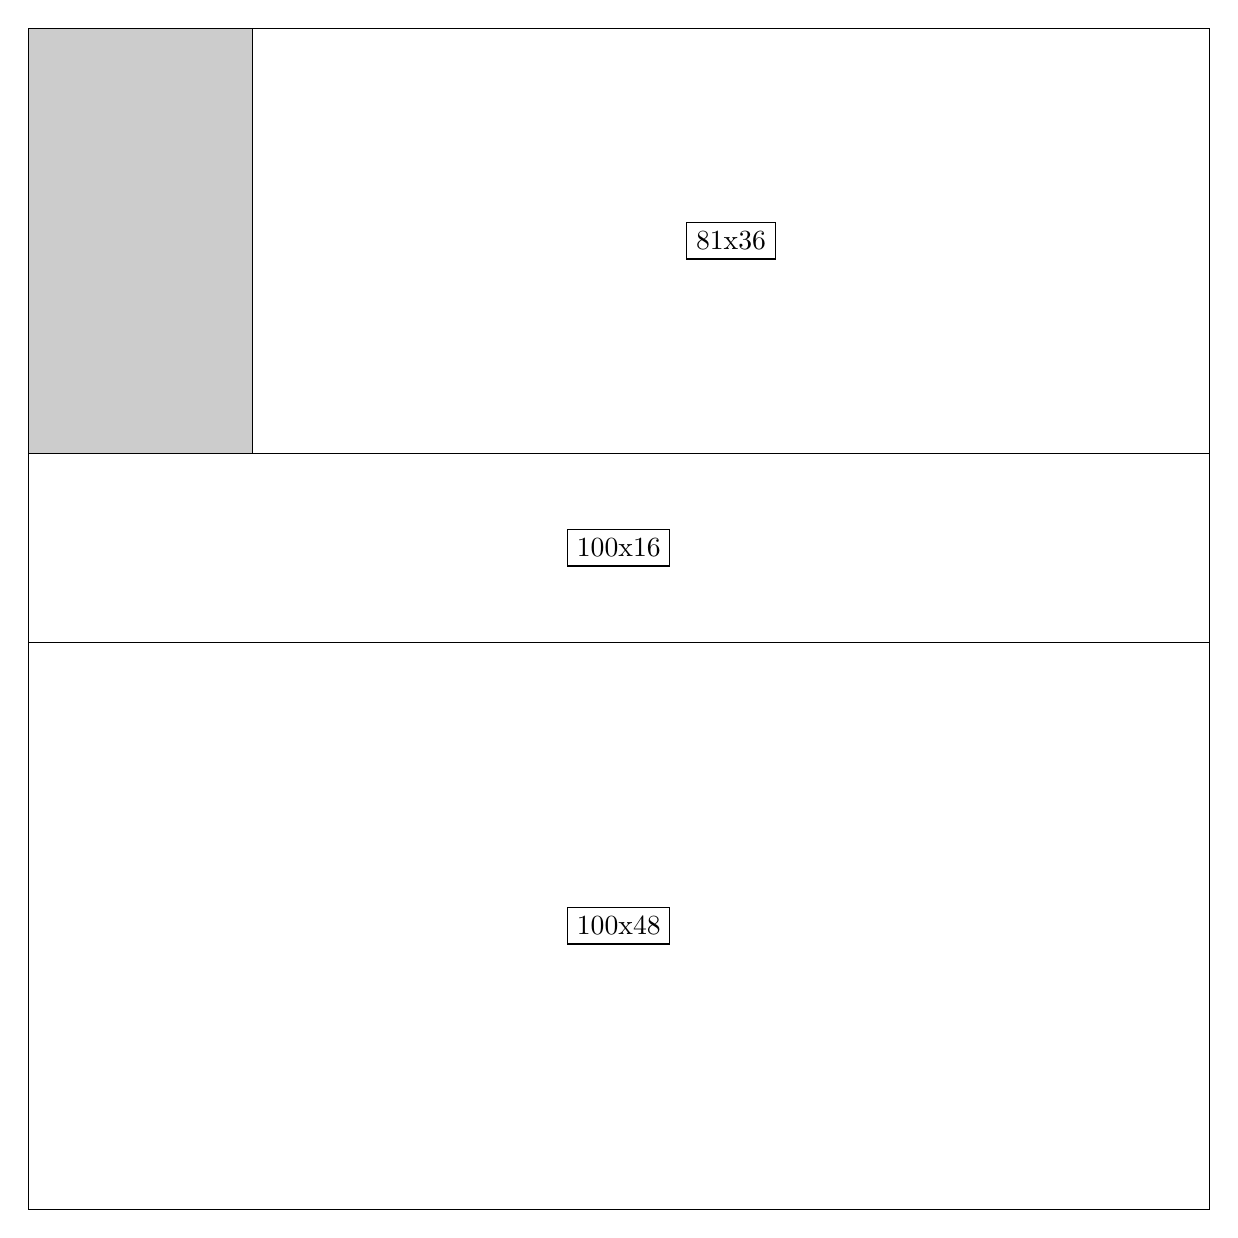
\begin{tikzpicture}[shorten >=1pt,scale=1.0,every node/.style={scale=1.0},->]
\tikzstyle{vertex}=[circle,fill=black!25,minimum size=14pt,inner sep=0pt]
\filldraw[fill=gray!40!white, draw=black] (0,0) rectangle (15.0,15.0);
\foreach \name/\x/\y/\w/\h in {100x48/0.0/0.0/15.0/7.199999999999999,100x16/0.0/7.199999999999999/15.0/2.4,81x36/2.85/9.6/12.15/5.3999999999999995}
\filldraw[fill=white!40!white, draw=black] (\x,\y) rectangle node[draw] (\name) {\name} ++(\w,\h);
\end{tikzpicture}


w =100 , h =48 , x =0 , y =0 , v =4800
\par
w =100 , h =16 , x =0 , y =48 , v =1600
\par
w =81 , h =36 , x =19 , y =64 , v =2916
\par
\newpage


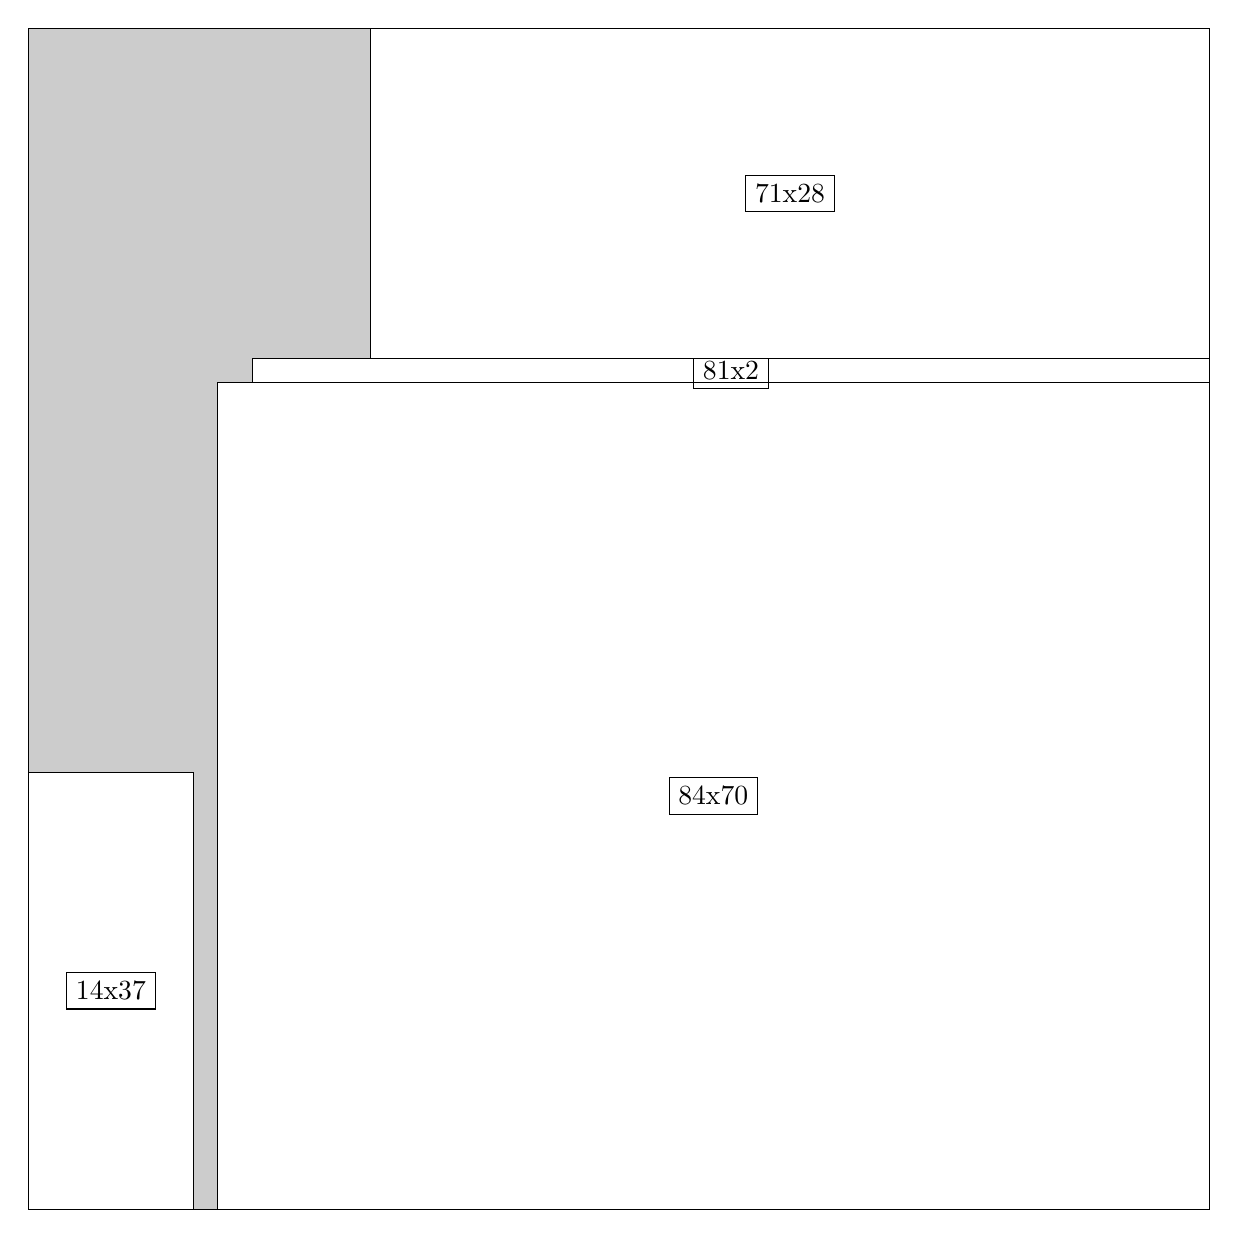
\begin{tikzpicture}[shorten >=1pt,scale=1.0,every node/.style={scale=1.0},->]
\tikzstyle{vertex}=[circle,fill=black!25,minimum size=14pt,inner sep=0pt]
\filldraw[fill=gray!40!white, draw=black] (0,0) rectangle (15.0,15.0);
\foreach \name/\x/\y/\w/\h in {84x70/2.4/0.0/12.6/10.5,81x2/2.85/10.5/12.15/0.3,71x28/4.35/10.799999999999999/10.65/4.2,14x37/0.0/0.0/2.1/5.55}
\filldraw[fill=white!40!white, draw=black] (\x,\y) rectangle node[draw] (\name) {\name} ++(\w,\h);
\end{tikzpicture}


w =84 , h =70 , x =16 , y =0 , v =5880
\par
w =81 , h =2 , x =19 , y =70 , v =162
\par
w =71 , h =28 , x =29 , y =72 , v =1988
\par
w =14 , h =37 , x =0 , y =0 , v =518
\par
\newpage


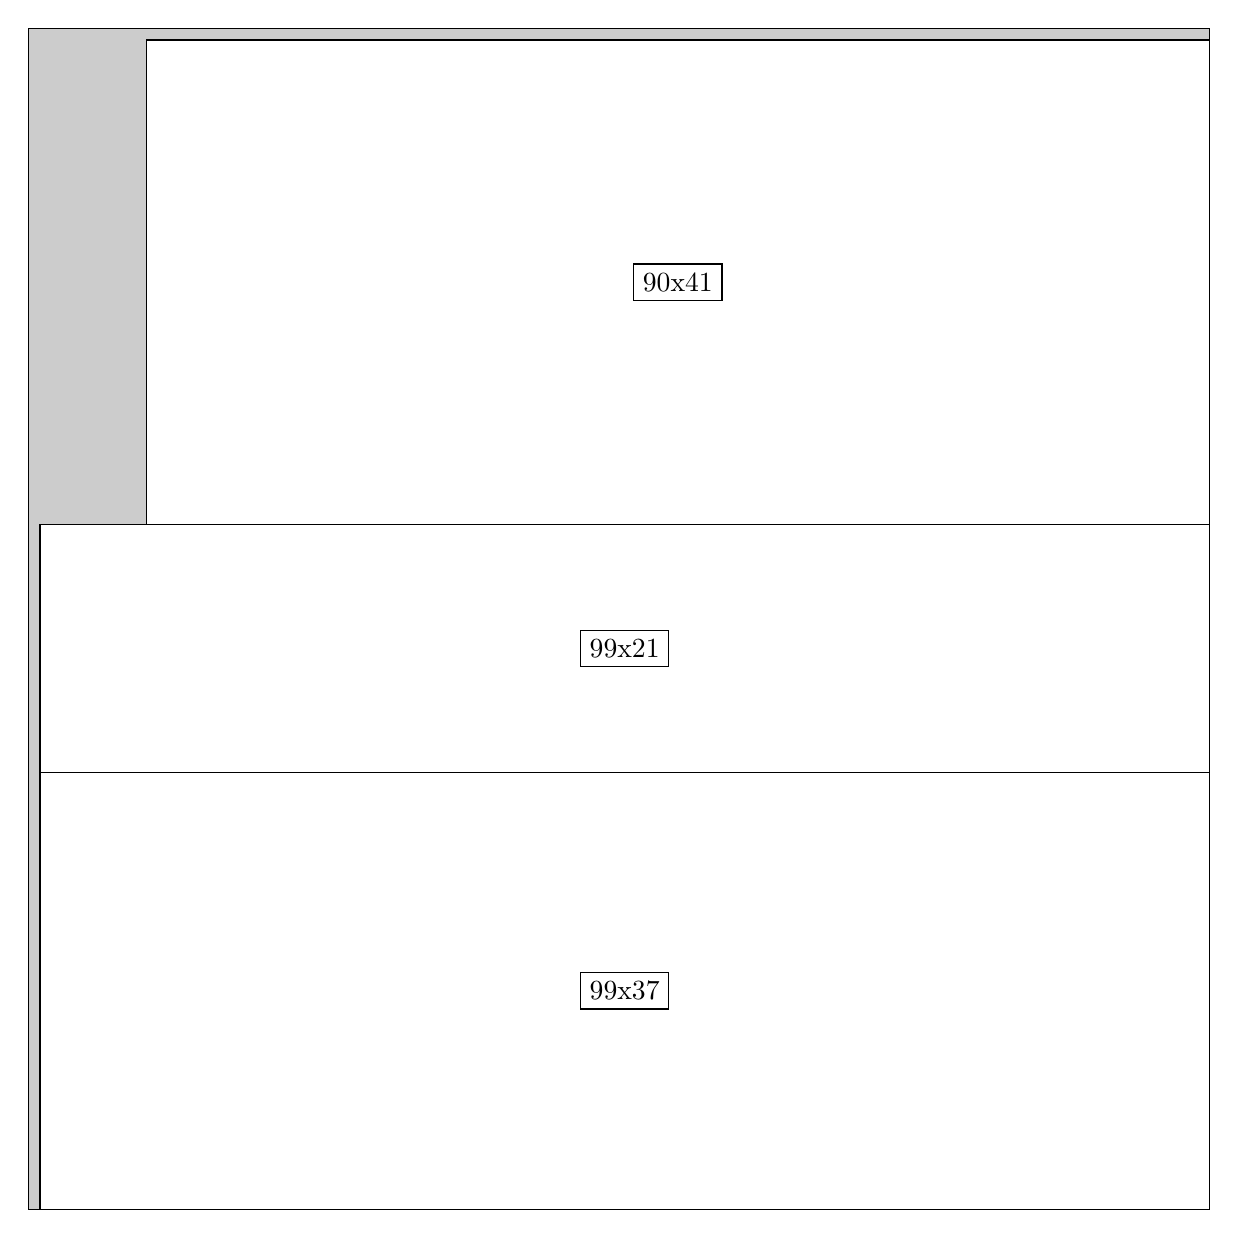
\begin{tikzpicture}[shorten >=1pt,scale=1.0,every node/.style={scale=1.0},->]
\tikzstyle{vertex}=[circle,fill=black!25,minimum size=14pt,inner sep=0pt]
\filldraw[fill=gray!40!white, draw=black] (0,0) rectangle (15.0,15.0);
\foreach \name/\x/\y/\w/\h in {99x37/0.15/0.0/14.85/5.55,99x21/0.15/5.55/14.85/3.15,90x41/1.5/8.7/13.5/6.1499999999999995}
\filldraw[fill=white!40!white, draw=black] (\x,\y) rectangle node[draw] (\name) {\name} ++(\w,\h);
\end{tikzpicture}


w =99 , h =37 , x =1 , y =0 , v =3663
\par
w =99 , h =21 , x =1 , y =37 , v =2079
\par
w =90 , h =41 , x =10 , y =58 , v =3690
\par
\newpage


\begin{tikzpicture}[shorten >=1pt,scale=1.0,every node/.style={scale=1.0},->]
\tikzstyle{vertex}=[circle,fill=black!25,minimum size=14pt,inner sep=0pt]
\filldraw[fill=gray!40!white, draw=black] (0,0) rectangle (15.0,15.0);
\foreach \name/\x/\y/\w/\h in {99x96/0.15/0.0/14.85/14.399999999999999,90x4/1.5/14.399999999999999/13.5/0.6}
\filldraw[fill=white!40!white, draw=black] (\x,\y) rectangle node[draw] (\name) {\name} ++(\w,\h);
\end{tikzpicture}


w =99 , h =96 , x =1 , y =0 , v =9504
\par
w =90 , h =4 , x =10 , y =96 , v =360
\par
\newpage


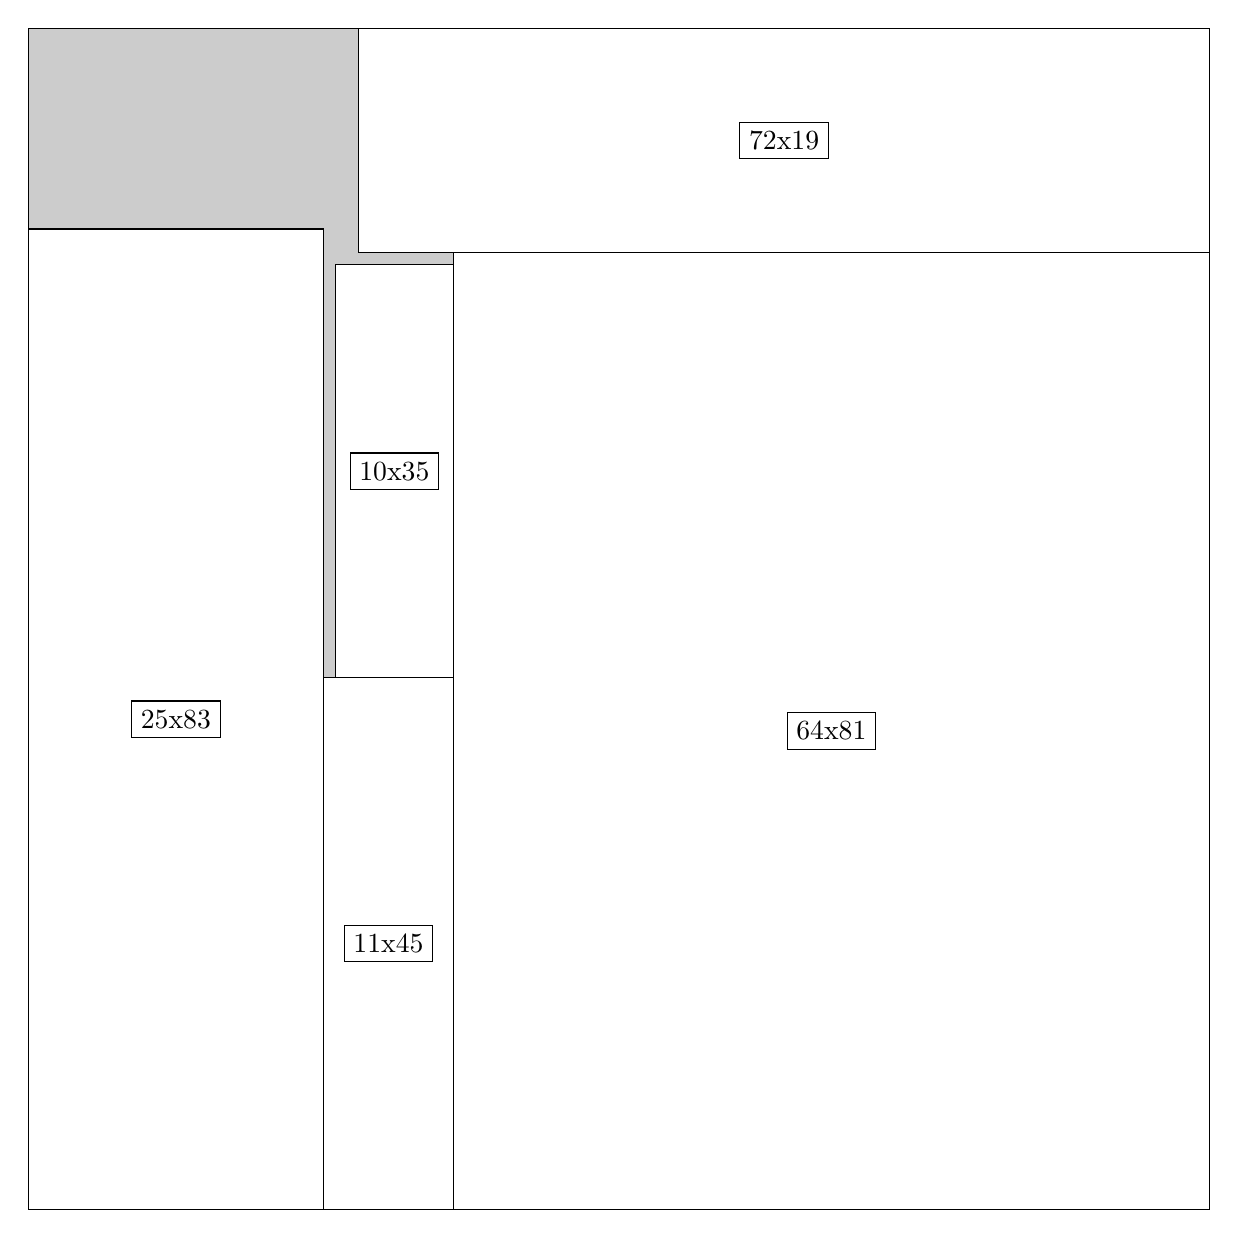
\begin{tikzpicture}[shorten >=1pt,scale=1.0,every node/.style={scale=1.0},->]
\tikzstyle{vertex}=[circle,fill=black!25,minimum size=14pt,inner sep=0pt]
\filldraw[fill=gray!40!white, draw=black] (0,0) rectangle (15.0,15.0);
\foreach \name/\x/\y/\w/\h in {64x81/5.3999999999999995/0.0/9.6/12.15,11x45/3.75/0.0/1.65/6.75,10x35/3.9/6.75/1.5/5.25,72x19/4.2/12.15/10.799999999999999/2.85,25x83/0.0/0.0/3.75/12.45}
\filldraw[fill=white!40!white, draw=black] (\x,\y) rectangle node[draw] (\name) {\name} ++(\w,\h);
\end{tikzpicture}


w =64 , h =81 , x =36 , y =0 , v =5184
\par
w =11 , h =45 , x =25 , y =0 , v =495
\par
w =10 , h =35 , x =26 , y =45 , v =350
\par
w =72 , h =19 , x =28 , y =81 , v =1368
\par
w =25 , h =83 , x =0 , y =0 , v =2075
\par
\newpage


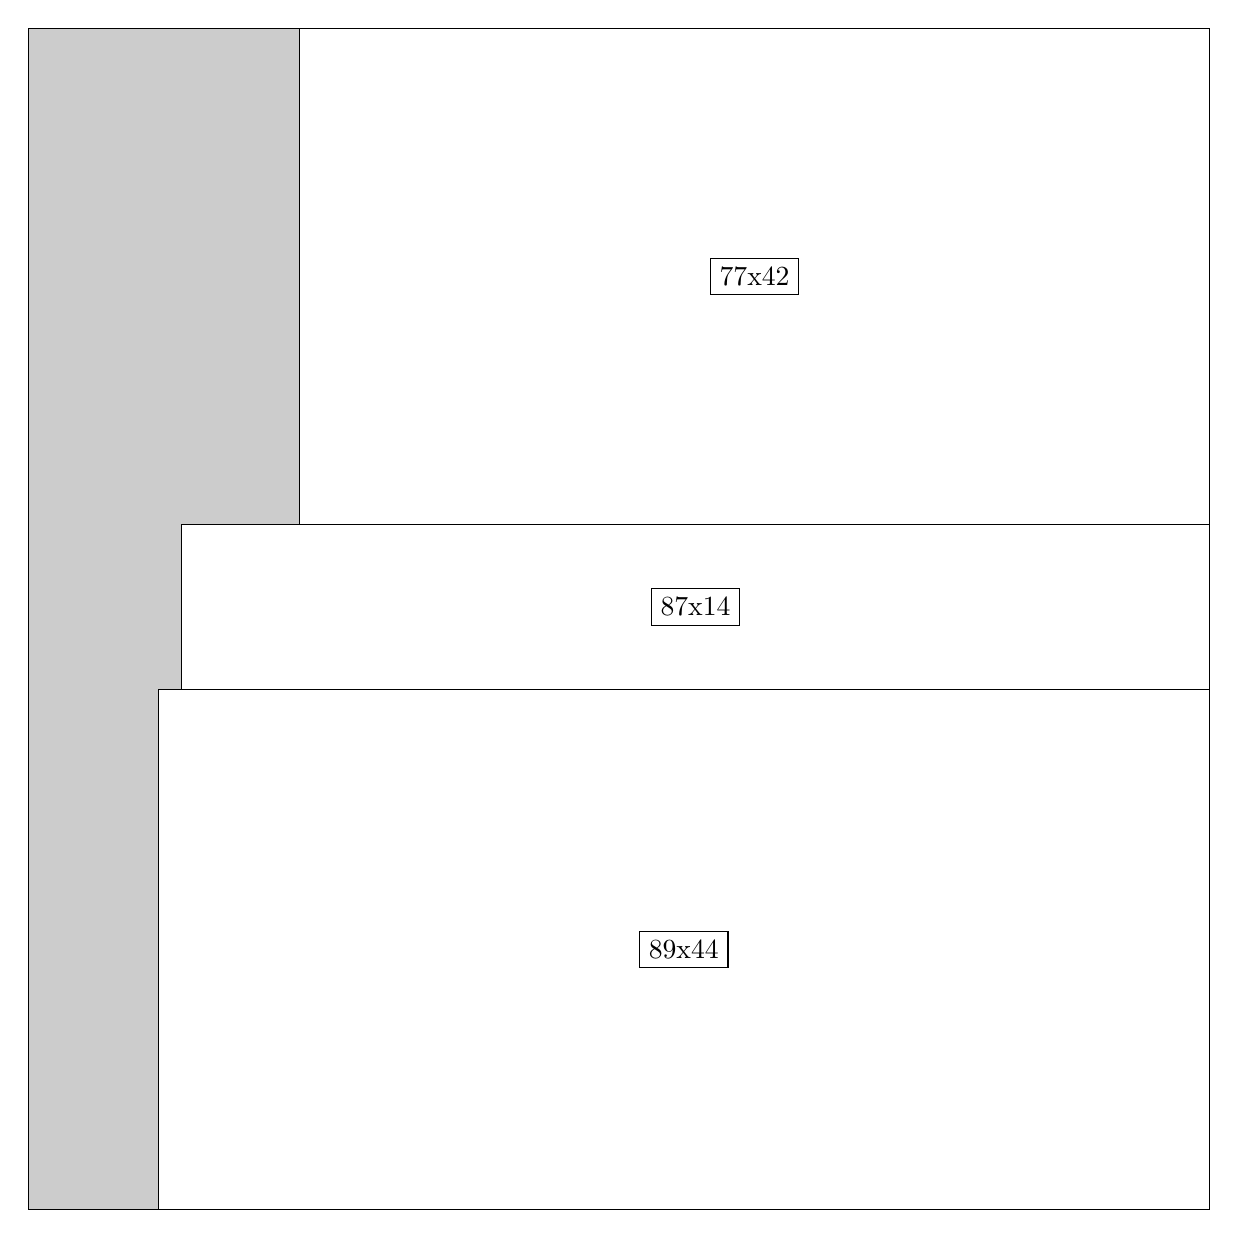
\begin{tikzpicture}[shorten >=1pt,scale=1.0,every node/.style={scale=1.0},->]
\tikzstyle{vertex}=[circle,fill=black!25,minimum size=14pt,inner sep=0pt]
\filldraw[fill=gray!40!white, draw=black] (0,0) rectangle (15.0,15.0);
\foreach \name/\x/\y/\w/\h in {89x44/1.65/0.0/13.35/6.6,87x14/1.95/6.6/13.049999999999999/2.1,77x42/3.4499999999999997/8.7/11.549999999999999/6.3}
\filldraw[fill=white!40!white, draw=black] (\x,\y) rectangle node[draw] (\name) {\name} ++(\w,\h);
\end{tikzpicture}


w =89 , h =44 , x =11 , y =0 , v =3916
\par
w =87 , h =14 , x =13 , y =44 , v =1218
\par
w =77 , h =42 , x =23 , y =58 , v =3234
\par
\newpage


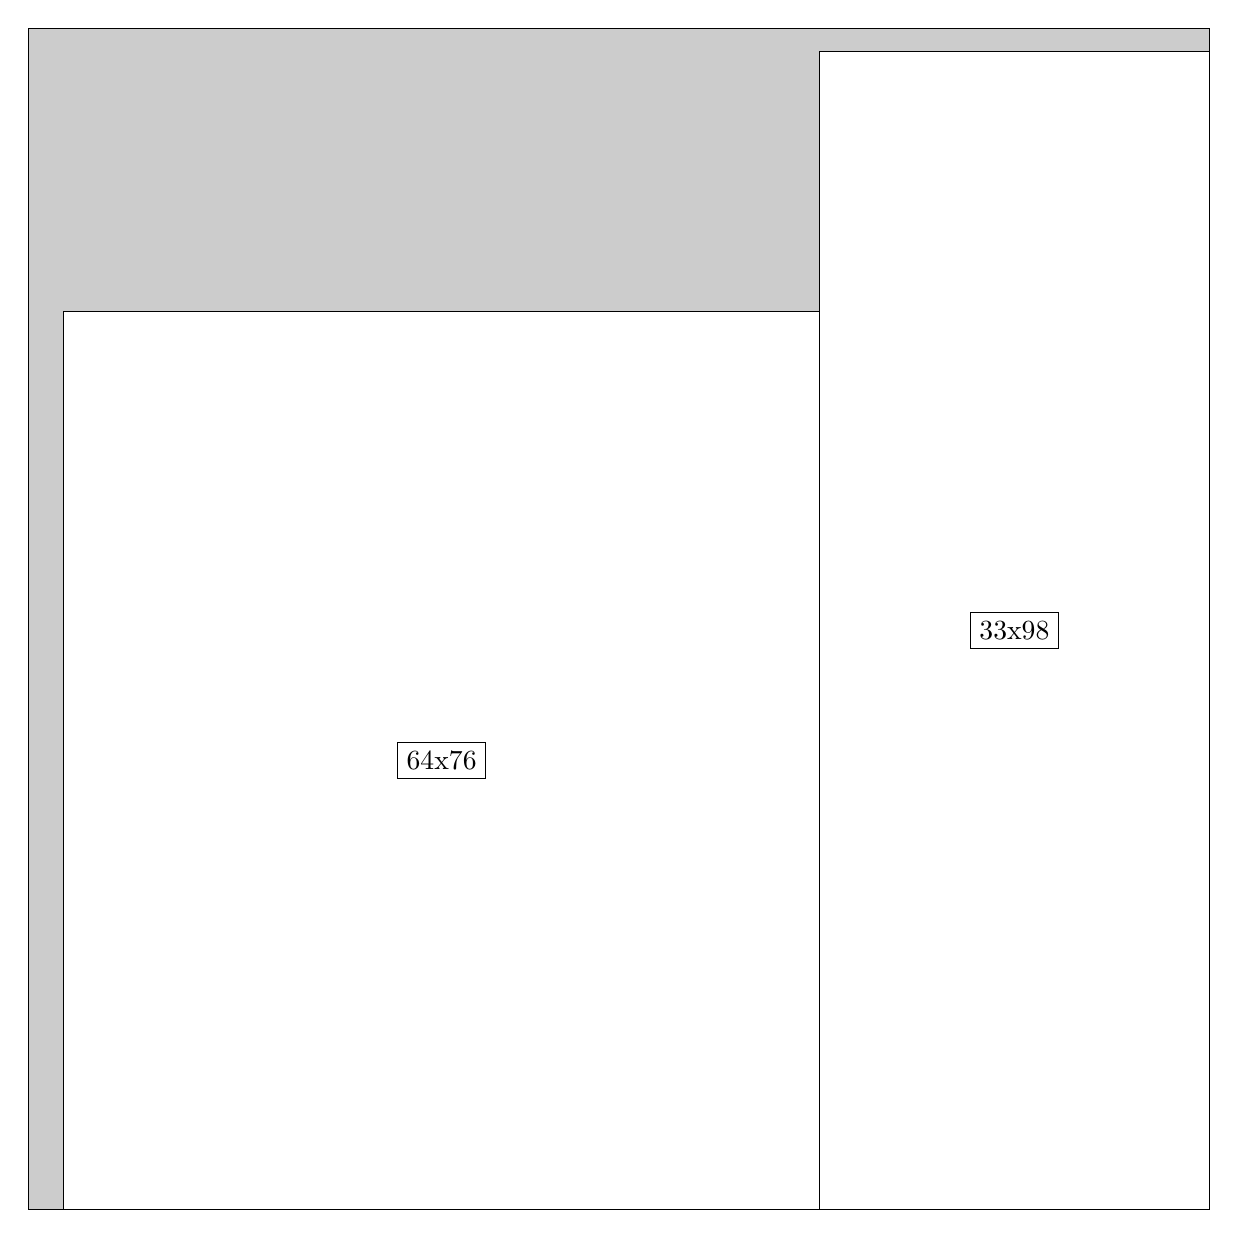
\begin{tikzpicture}[shorten >=1pt,scale=1.0,every node/.style={scale=1.0},->]
\tikzstyle{vertex}=[circle,fill=black!25,minimum size=14pt,inner sep=0pt]
\filldraw[fill=gray!40!white, draw=black] (0,0) rectangle (15.0,15.0);
\foreach \name/\x/\y/\w/\h in {33x98/10.049999999999999/0.0/4.95/14.7,64x76/0.44999999999999996/0.0/9.6/11.4}
\filldraw[fill=white!40!white, draw=black] (\x,\y) rectangle node[draw] (\name) {\name} ++(\w,\h);
\end{tikzpicture}


w =33 , h =98 , x =67 , y =0 , v =3234
\par
w =64 , h =76 , x =3 , y =0 , v =4864
\par
\newpage


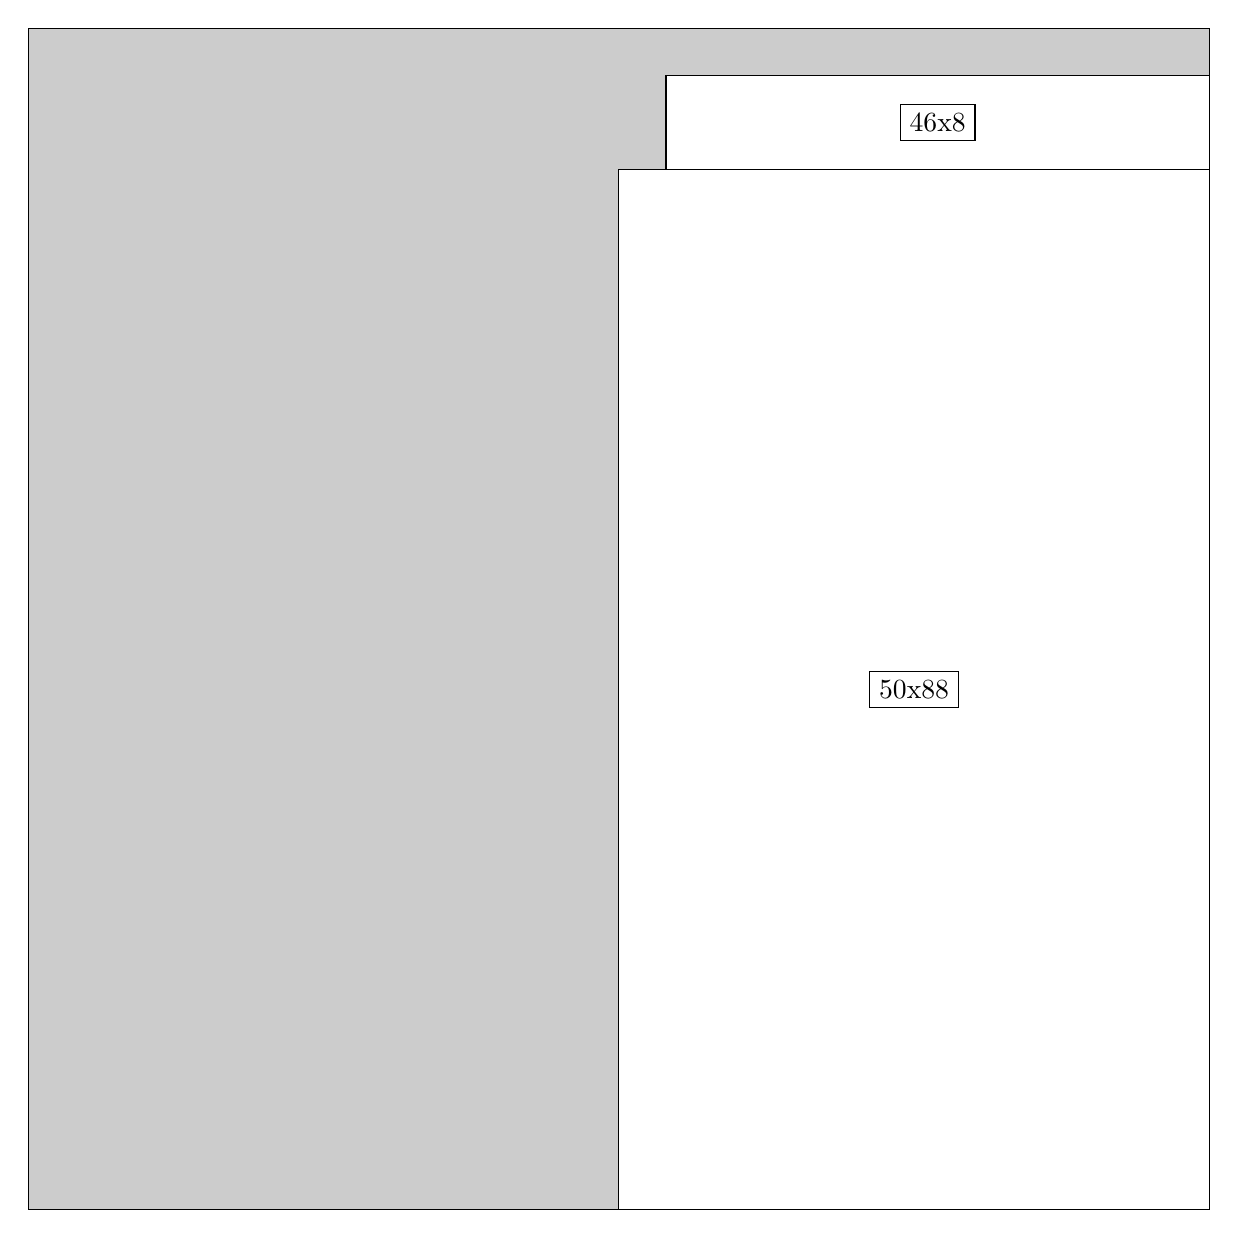
\begin{tikzpicture}[shorten >=1pt,scale=1.0,every node/.style={scale=1.0},->]
\tikzstyle{vertex}=[circle,fill=black!25,minimum size=14pt,inner sep=0pt]
\filldraw[fill=gray!40!white, draw=black] (0,0) rectangle (15.0,15.0);
\foreach \name/\x/\y/\w/\h in {50x88/7.5/0.0/7.5/13.2,46x8/8.1/13.2/6.8999999999999995/1.2}
\filldraw[fill=white!40!white, draw=black] (\x,\y) rectangle node[draw] (\name) {\name} ++(\w,\h);
\end{tikzpicture}


w =50 , h =88 , x =50 , y =0 , v =4400
\par
w =46 , h =8 , x =54 , y =88 , v =368
\par
\newpage


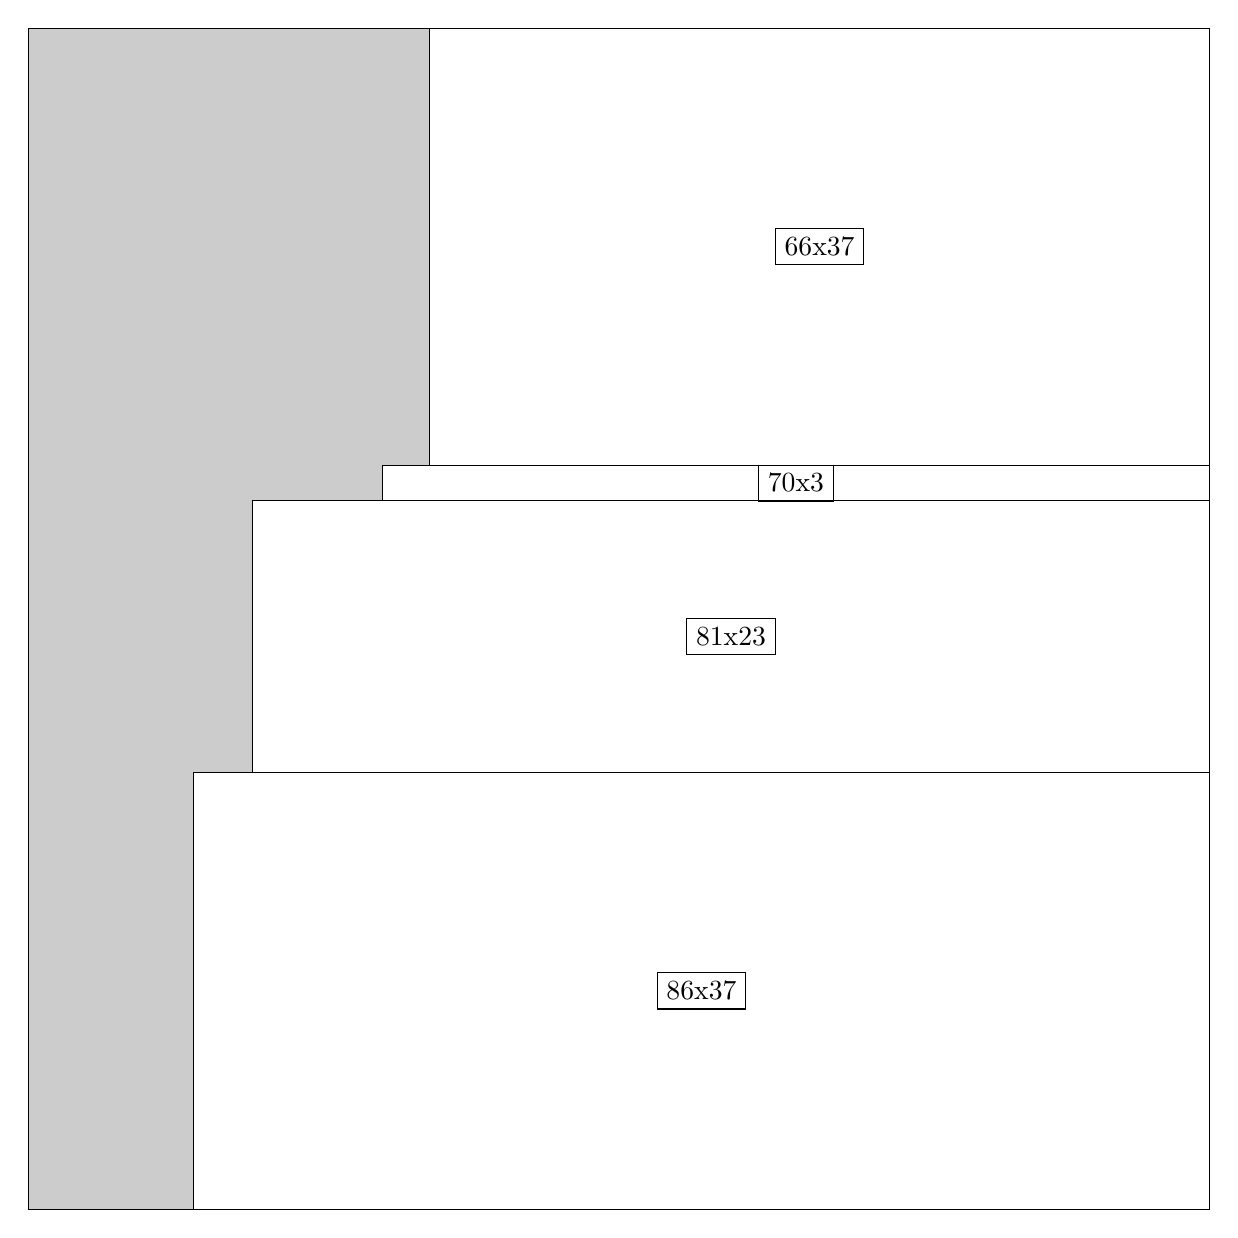
\begin{tikzpicture}[shorten >=1pt,scale=1.0,every node/.style={scale=1.0},->]
\tikzstyle{vertex}=[circle,fill=black!25,minimum size=14pt,inner sep=0pt]
\filldraw[fill=gray!40!white, draw=black] (0,0) rectangle (15.0,15.0);
\foreach \name/\x/\y/\w/\h in {86x37/2.1/0.0/12.9/5.55,81x23/2.85/5.55/12.15/3.4499999999999997,70x3/4.5/9.0/10.5/0.44999999999999996,66x37/5.1/9.45/9.9/5.55}
\filldraw[fill=white!40!white, draw=black] (\x,\y) rectangle node[draw] (\name) {\name} ++(\w,\h);
\end{tikzpicture}


w =86 , h =37 , x =14 , y =0 , v =3182
\par
w =81 , h =23 , x =19 , y =37 , v =1863
\par
w =70 , h =3 , x =30 , y =60 , v =210
\par
w =66 , h =37 , x =34 , y =63 , v =2442
\par
\newpage


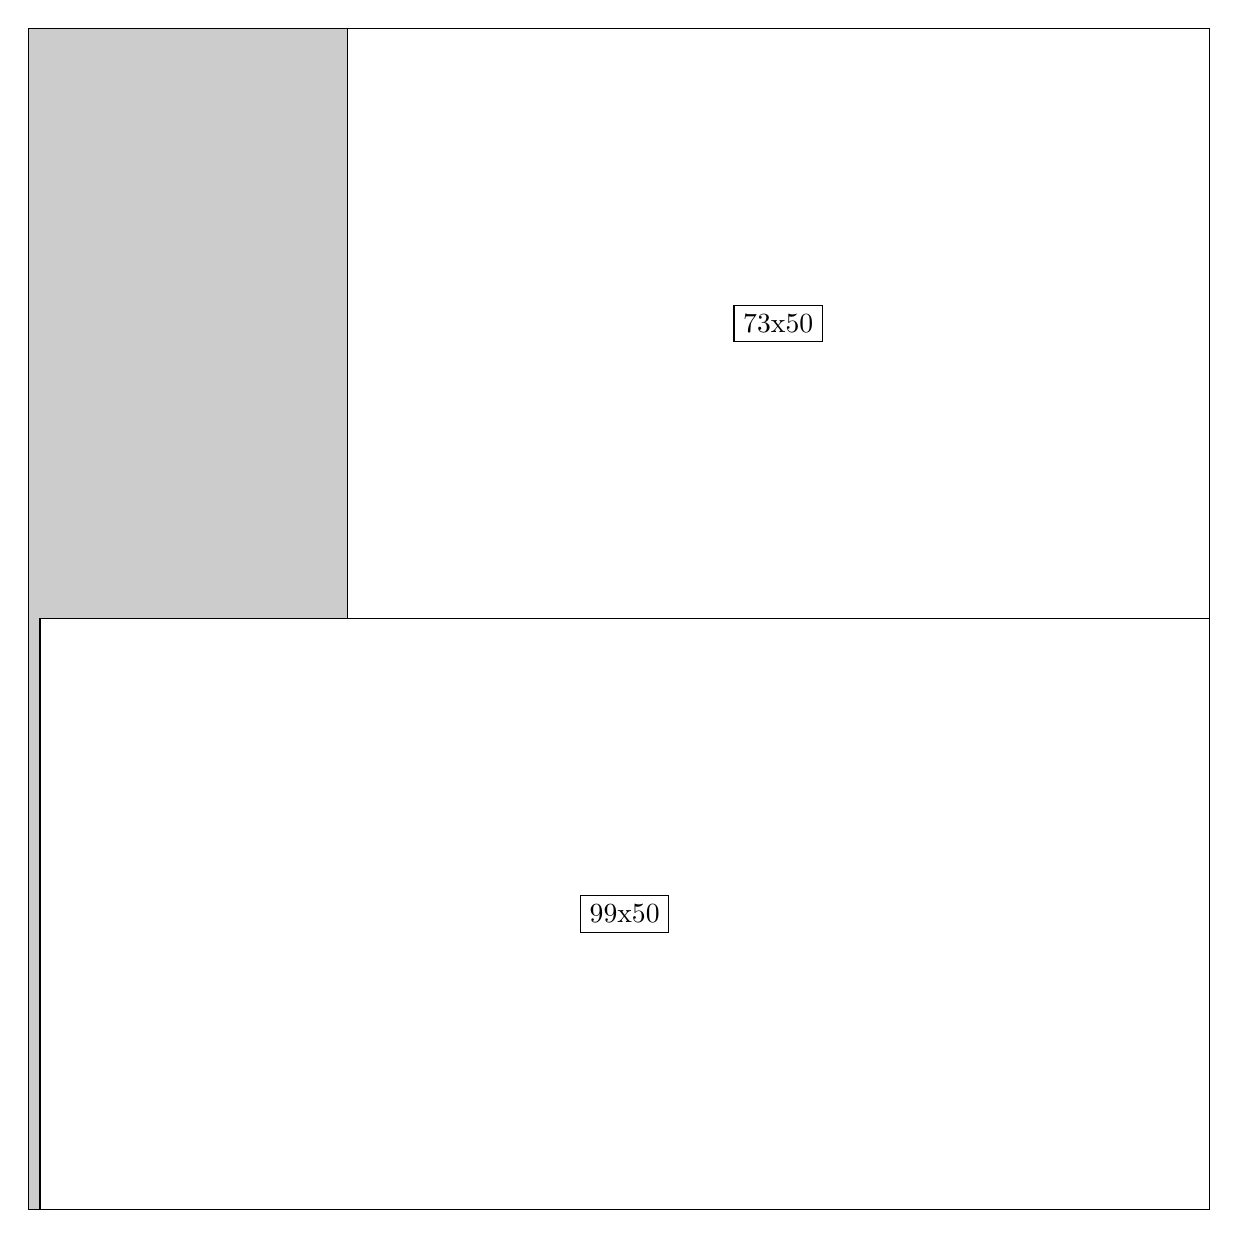
\begin{tikzpicture}[shorten >=1pt,scale=1.0,every node/.style={scale=1.0},->]
\tikzstyle{vertex}=[circle,fill=black!25,minimum size=14pt,inner sep=0pt]
\filldraw[fill=gray!40!white, draw=black] (0,0) rectangle (15.0,15.0);
\foreach \name/\x/\y/\w/\h in {99x50/0.15/0.0/14.85/7.5,73x50/4.05/7.5/10.95/7.5}
\filldraw[fill=white!40!white, draw=black] (\x,\y) rectangle node[draw] (\name) {\name} ++(\w,\h);
\end{tikzpicture}


w =99 , h =50 , x =1 , y =0 , v =4950
\par
w =73 , h =50 , x =27 , y =50 , v =3650
\par
\newpage


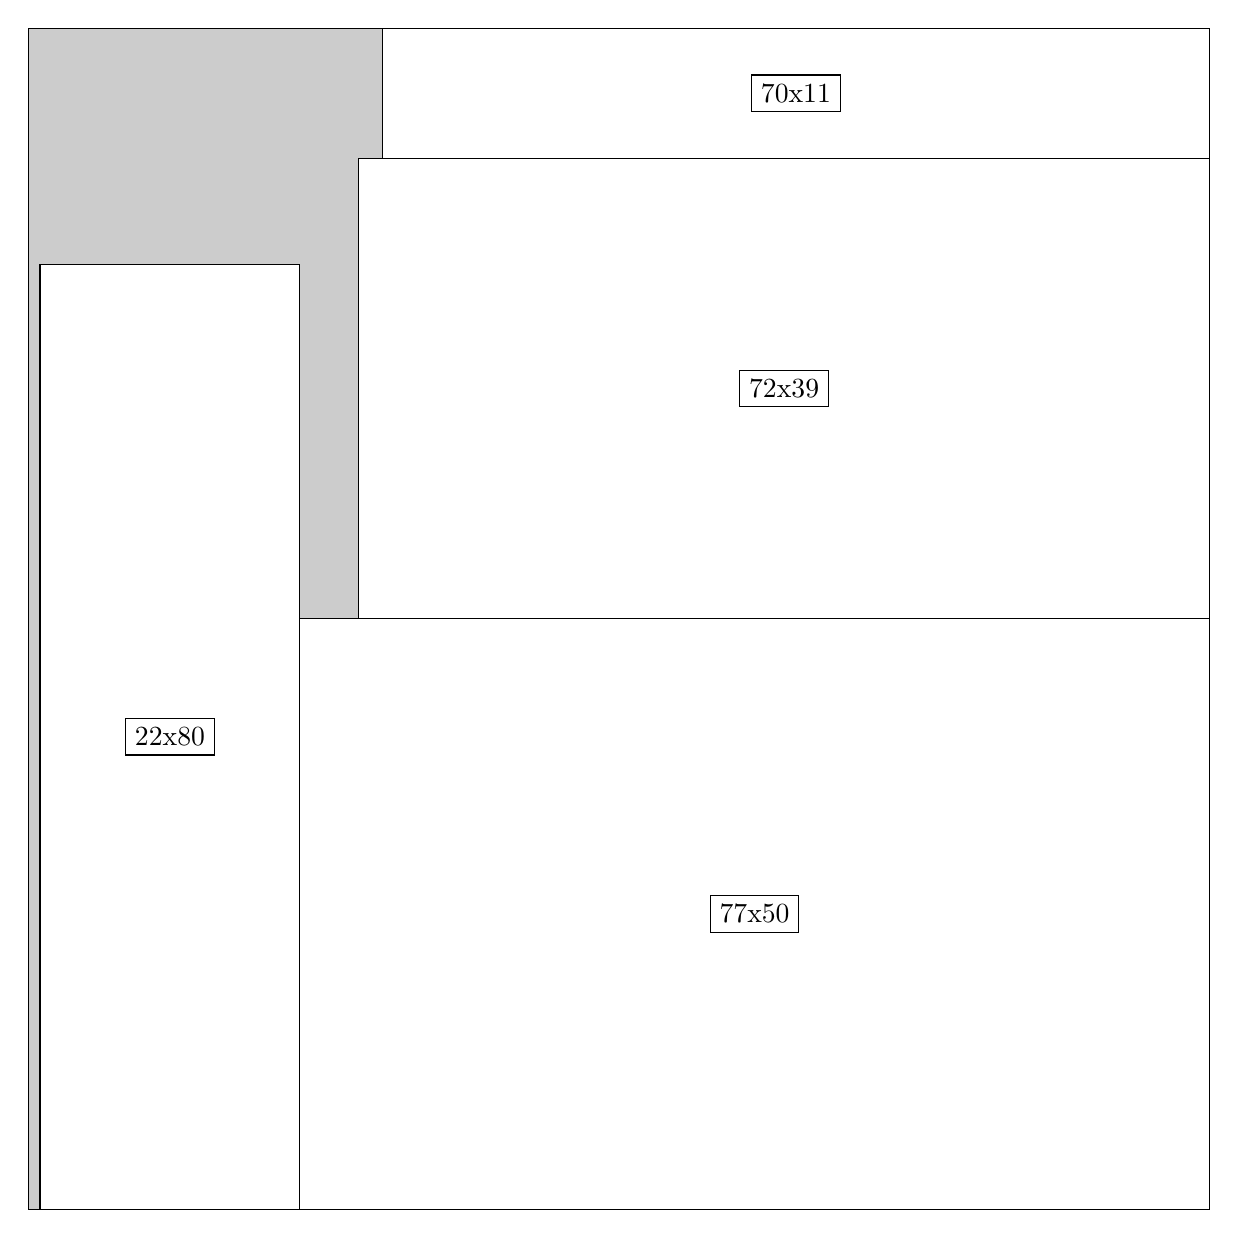
\begin{tikzpicture}[shorten >=1pt,scale=1.0,every node/.style={scale=1.0},->]
\tikzstyle{vertex}=[circle,fill=black!25,minimum size=14pt,inner sep=0pt]
\filldraw[fill=gray!40!white, draw=black] (0,0) rectangle (15.0,15.0);
\foreach \name/\x/\y/\w/\h in {77x50/3.4499999999999997/0.0/11.549999999999999/7.5,72x39/4.2/7.5/10.799999999999999/5.85,70x11/4.5/13.35/10.5/1.65,22x80/0.15/0.0/3.3/12.0}
\filldraw[fill=white!40!white, draw=black] (\x,\y) rectangle node[draw] (\name) {\name} ++(\w,\h);
\end{tikzpicture}


w =77 , h =50 , x =23 , y =0 , v =3850
\par
w =72 , h =39 , x =28 , y =50 , v =2808
\par
w =70 , h =11 , x =30 , y =89 , v =770
\par
w =22 , h =80 , x =1 , y =0 , v =1760
\par
\newpage


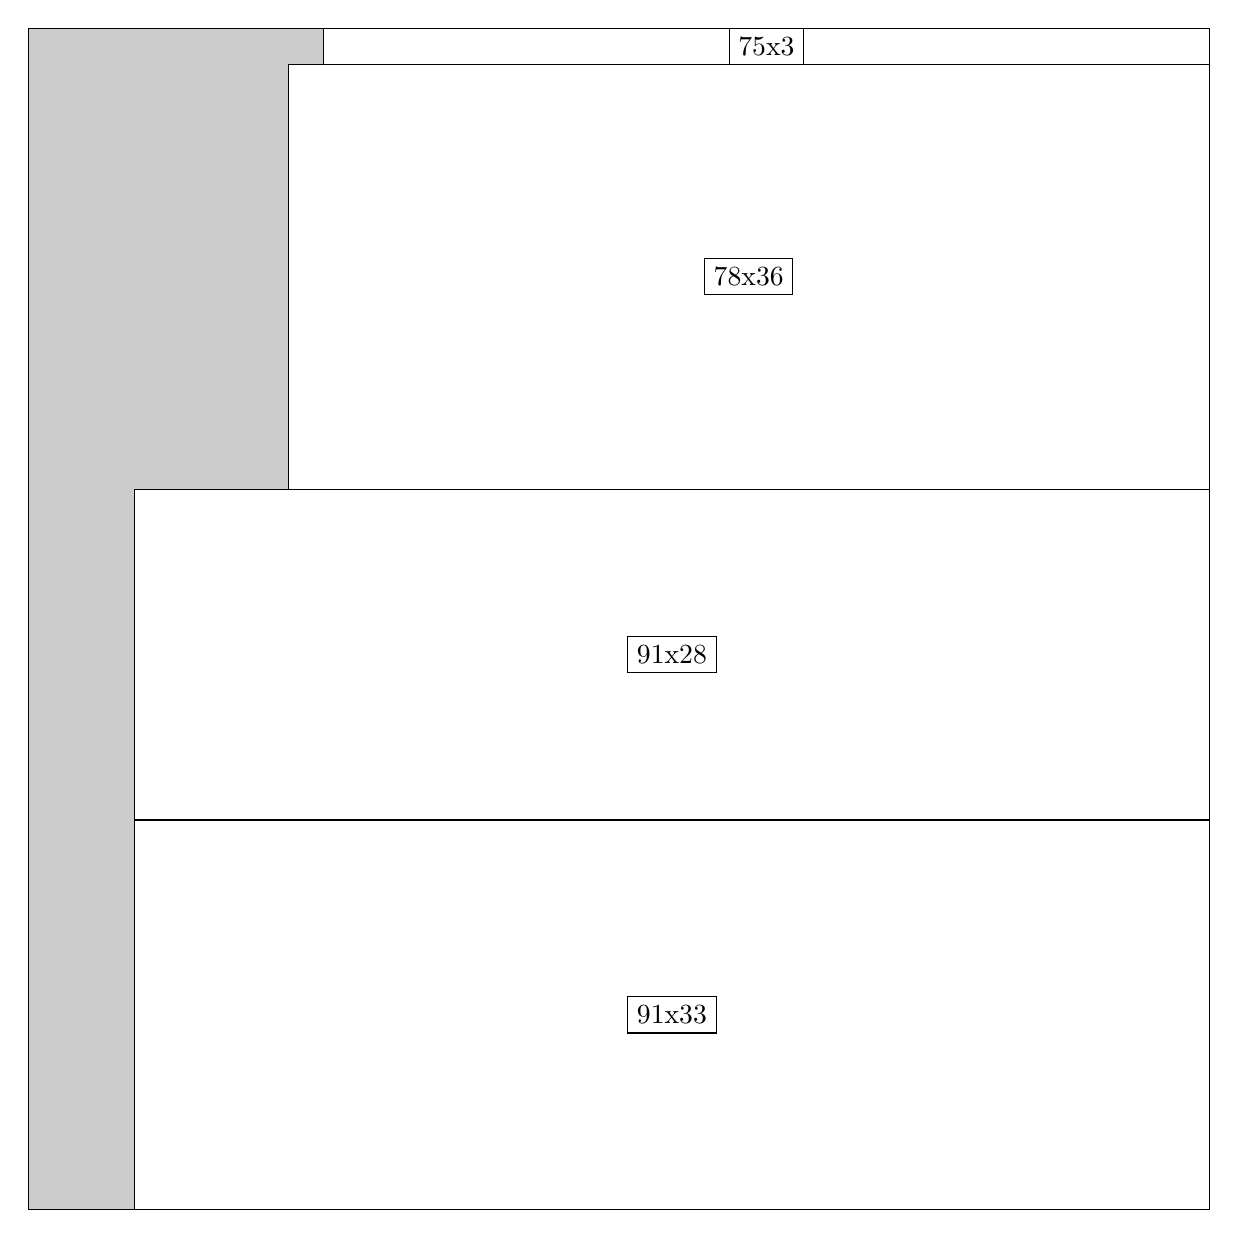
\begin{tikzpicture}[shorten >=1pt,scale=1.0,every node/.style={scale=1.0},->]
\tikzstyle{vertex}=[circle,fill=black!25,minimum size=14pt,inner sep=0pt]
\filldraw[fill=gray!40!white, draw=black] (0,0) rectangle (15.0,15.0);
\foreach \name/\x/\y/\w/\h in {91x33/1.3499999999999999/0.0/13.65/4.95,91x28/1.3499999999999999/4.95/13.65/4.2,78x36/3.3/9.15/11.7/5.3999999999999995,75x3/3.75/14.549999999999999/11.25/0.44999999999999996}
\filldraw[fill=white!40!white, draw=black] (\x,\y) rectangle node[draw] (\name) {\name} ++(\w,\h);
\end{tikzpicture}


w =91 , h =33 , x =9 , y =0 , v =3003
\par
w =91 , h =28 , x =9 , y =33 , v =2548
\par
w =78 , h =36 , x =22 , y =61 , v =2808
\par
w =75 , h =3 , x =25 , y =97 , v =225
\par
\newpage


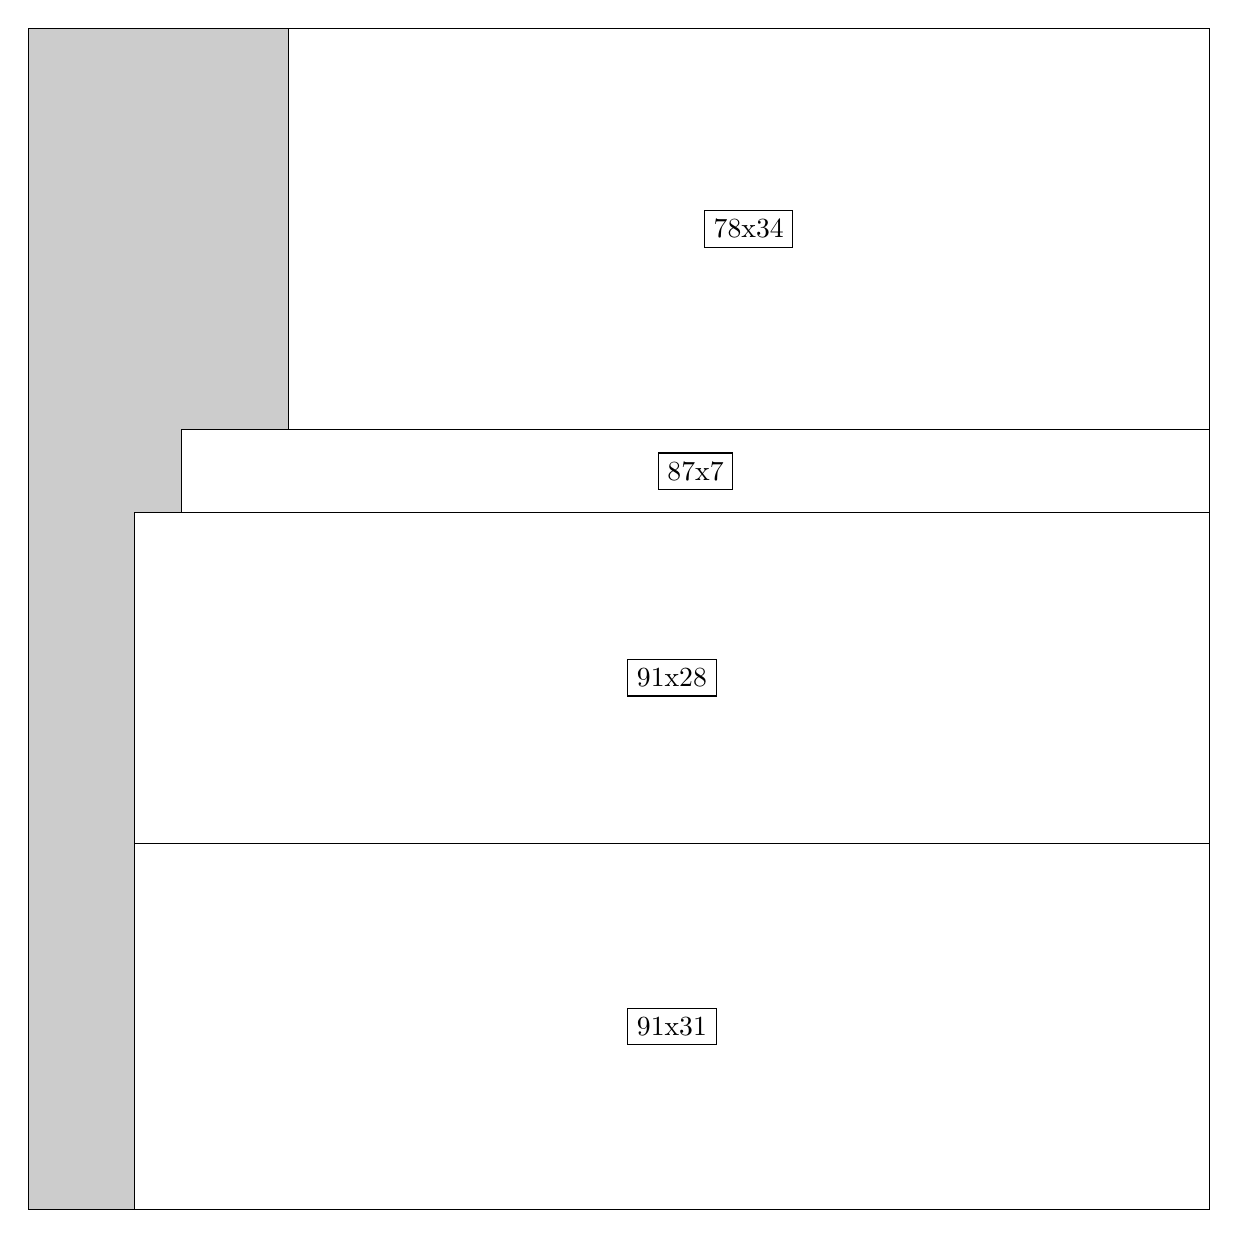
\begin{tikzpicture}[shorten >=1pt,scale=1.0,every node/.style={scale=1.0},->]
\tikzstyle{vertex}=[circle,fill=black!25,minimum size=14pt,inner sep=0pt]
\filldraw[fill=gray!40!white, draw=black] (0,0) rectangle (15.0,15.0);
\foreach \name/\x/\y/\w/\h in {91x31/1.3499999999999999/0.0/13.65/4.6499999999999995,91x28/1.3499999999999999/4.6499999999999995/13.65/4.2,87x7/1.95/8.85/13.049999999999999/1.05,78x34/3.3/9.9/11.7/5.1}
\filldraw[fill=white!40!white, draw=black] (\x,\y) rectangle node[draw] (\name) {\name} ++(\w,\h);
\end{tikzpicture}


w =91 , h =31 , x =9 , y =0 , v =2821
\par
w =91 , h =28 , x =9 , y =31 , v =2548
\par
w =87 , h =7 , x =13 , y =59 , v =609
\par
w =78 , h =34 , x =22 , y =66 , v =2652
\par
\newpage


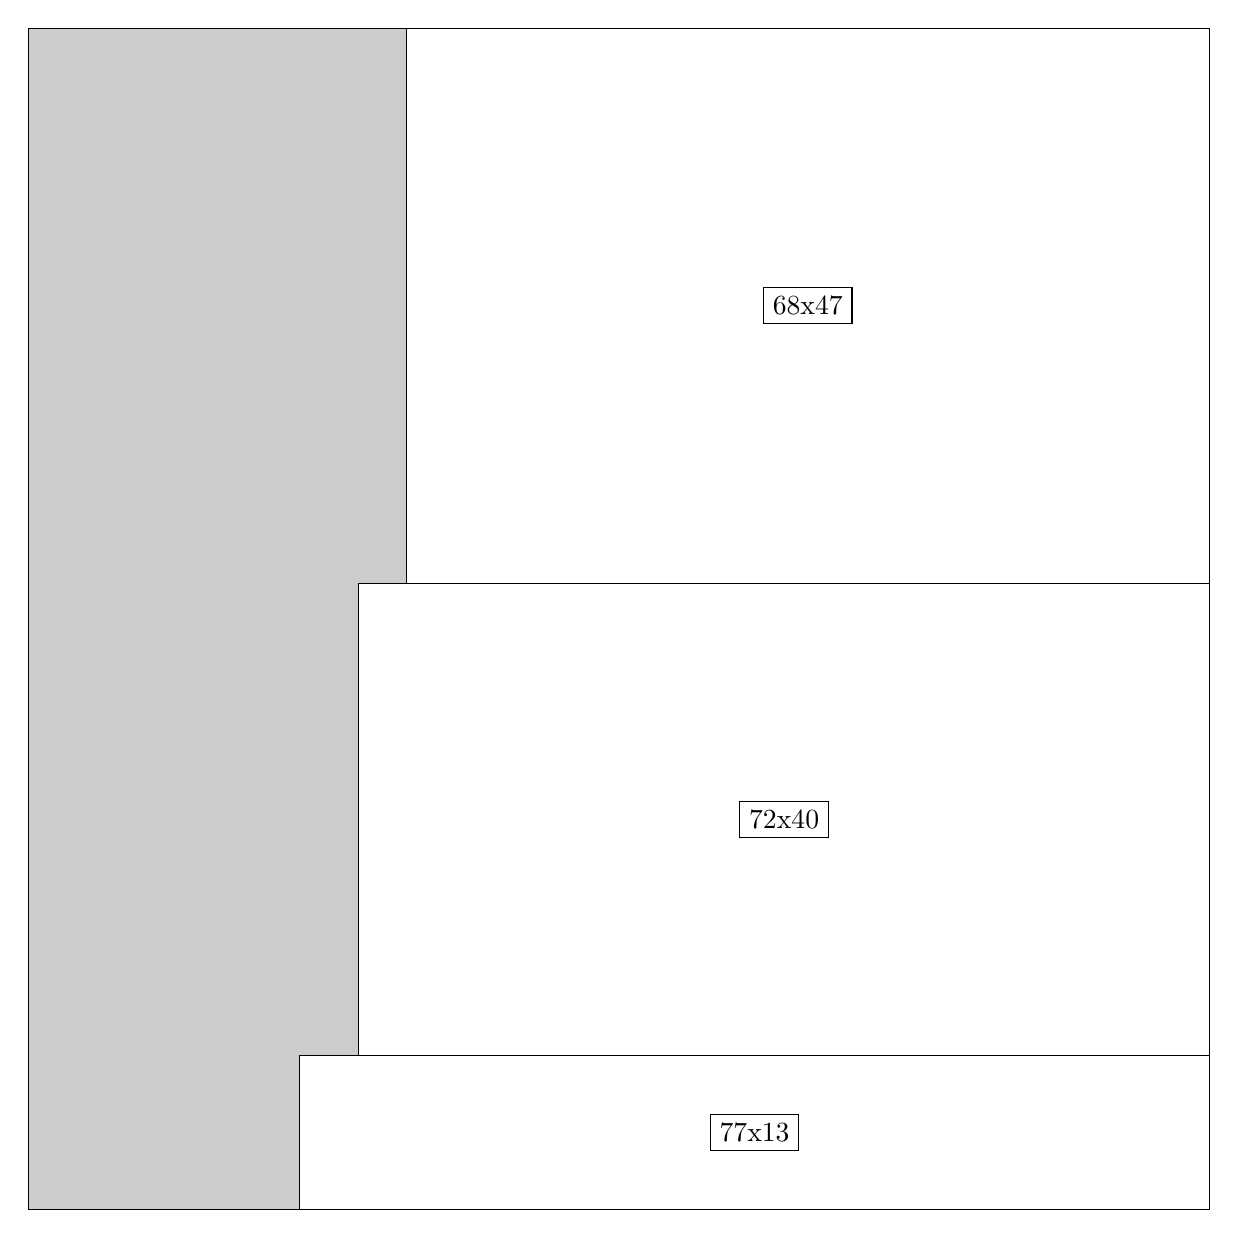
\begin{tikzpicture}[shorten >=1pt,scale=1.0,every node/.style={scale=1.0},->]
\tikzstyle{vertex}=[circle,fill=black!25,minimum size=14pt,inner sep=0pt]
\filldraw[fill=gray!40!white, draw=black] (0,0) rectangle (15.0,15.0);
\foreach \name/\x/\y/\w/\h in {77x13/3.4499999999999997/0.0/11.549999999999999/1.95,72x40/4.2/1.95/10.799999999999999/6.0,68x47/4.8/7.949999999999999/10.2/7.05}
\filldraw[fill=white!40!white, draw=black] (\x,\y) rectangle node[draw] (\name) {\name} ++(\w,\h);
\end{tikzpicture}


w =77 , h =13 , x =23 , y =0 , v =1001
\par
w =72 , h =40 , x =28 , y =13 , v =2880
\par
w =68 , h =47 , x =32 , y =53 , v =3196
\par
\newpage


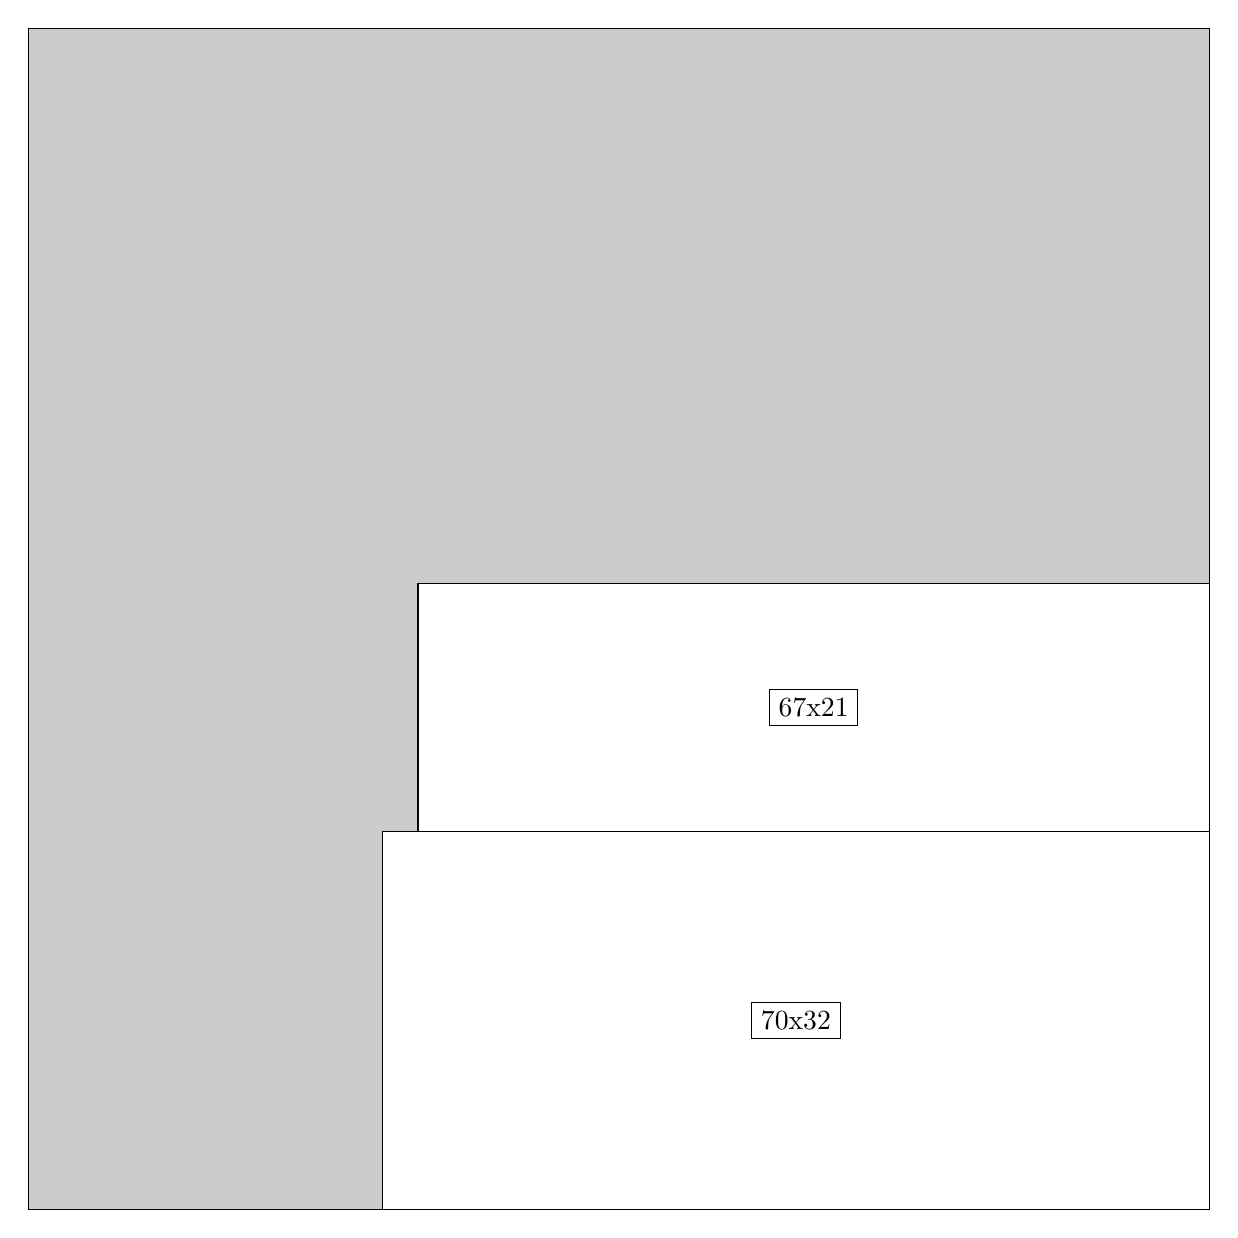
\begin{tikzpicture}[shorten >=1pt,scale=1.0,every node/.style={scale=1.0},->]
\tikzstyle{vertex}=[circle,fill=black!25,minimum size=14pt,inner sep=0pt]
\filldraw[fill=gray!40!white, draw=black] (0,0) rectangle (15.0,15.0);
\foreach \name/\x/\y/\w/\h in {70x32/4.5/0.0/10.5/4.8,67x21/4.95/4.8/10.049999999999999/3.15}
\filldraw[fill=white!40!white, draw=black] (\x,\y) rectangle node[draw] (\name) {\name} ++(\w,\h);
\end{tikzpicture}


w =70 , h =32 , x =30 , y =0 , v =2240
\par
w =67 , h =21 , x =33 , y =32 , v =1407
\par
\newpage


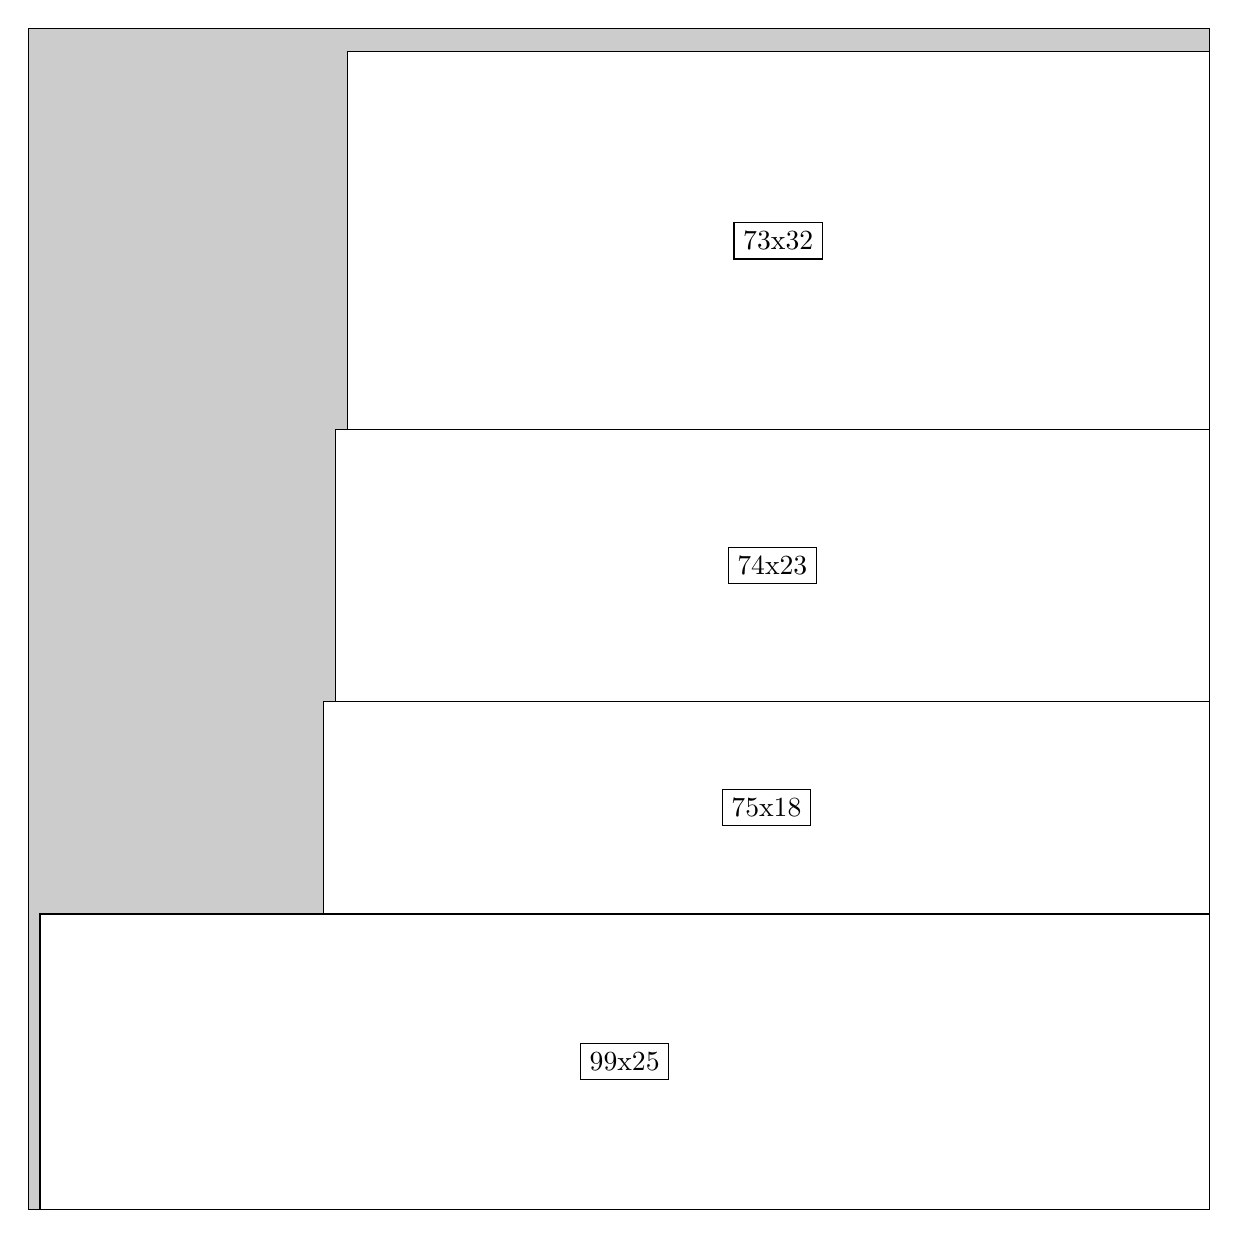
\begin{tikzpicture}[shorten >=1pt,scale=1.0,every node/.style={scale=1.0},->]
\tikzstyle{vertex}=[circle,fill=black!25,minimum size=14pt,inner sep=0pt]
\filldraw[fill=gray!40!white, draw=black] (0,0) rectangle (15.0,15.0);
\foreach \name/\x/\y/\w/\h in {99x25/0.15/0.0/14.85/3.75,75x18/3.75/3.75/11.25/2.6999999999999997,74x23/3.9/6.45/11.1/3.4499999999999997,73x32/4.05/9.9/10.95/4.8}
\filldraw[fill=white!40!white, draw=black] (\x,\y) rectangle node[draw] (\name) {\name} ++(\w,\h);
\end{tikzpicture}


w =99 , h =25 , x =1 , y =0 , v =2475
\par
w =75 , h =18 , x =25 , y =25 , v =1350
\par
w =74 , h =23 , x =26 , y =43 , v =1702
\par
w =73 , h =32 , x =27 , y =66 , v =2336
\par
\newpage


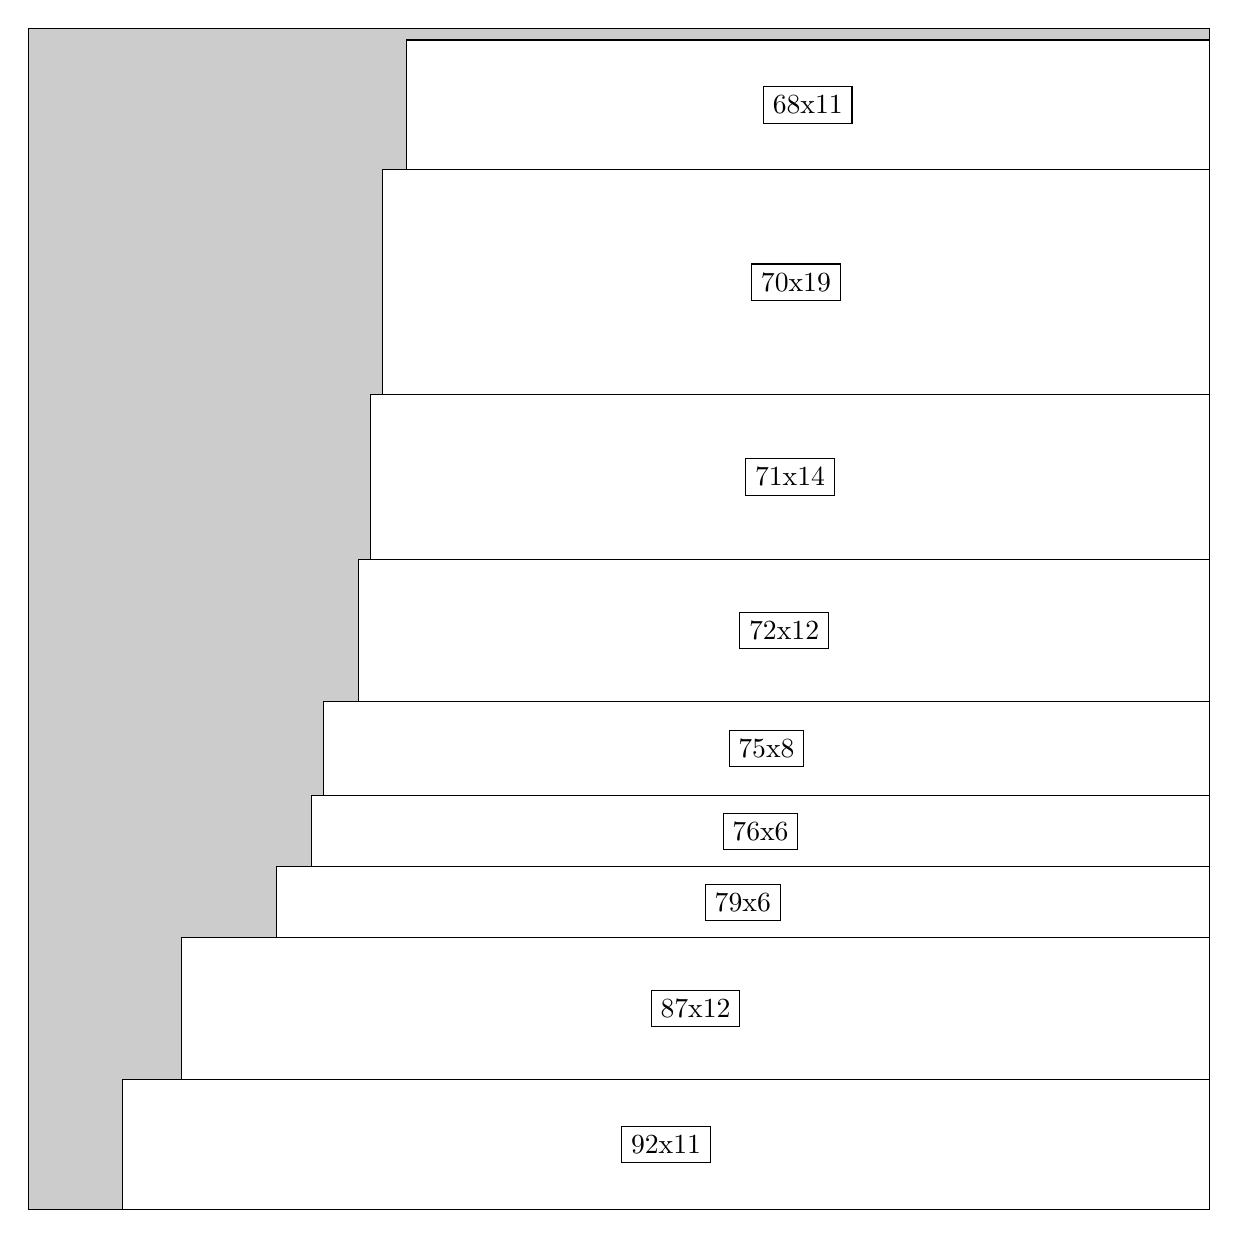
\begin{tikzpicture}[shorten >=1pt,scale=1.0,every node/.style={scale=1.0},->]
\tikzstyle{vertex}=[circle,fill=black!25,minimum size=14pt,inner sep=0pt]
\filldraw[fill=gray!40!white, draw=black] (0,0) rectangle (15.0,15.0);
\foreach \name/\x/\y/\w/\h in {92x11/1.2/0.0/13.799999999999999/1.65,87x12/1.95/1.65/13.049999999999999/1.7999999999999998,79x6/3.15/3.4499999999999997/11.85/0.8999999999999999,76x6/3.5999999999999996/4.35/11.4/0.8999999999999999,75x8/3.75/5.25/11.25/1.2,72x12/4.2/6.45/10.799999999999999/1.7999999999999998,71x14/4.35/8.25/10.65/2.1,70x19/4.5/10.35/10.5/2.85,68x11/4.8/13.2/10.2/1.65}
\filldraw[fill=white!40!white, draw=black] (\x,\y) rectangle node[draw] (\name) {\name} ++(\w,\h);
\end{tikzpicture}


w =92 , h =11 , x =8 , y =0 , v =1012
\par
w =87 , h =12 , x =13 , y =11 , v =1044
\par
w =79 , h =6 , x =21 , y =23 , v =474
\par
w =76 , h =6 , x =24 , y =29 , v =456
\par
w =75 , h =8 , x =25 , y =35 , v =600
\par
w =72 , h =12 , x =28 , y =43 , v =864
\par
w =71 , h =14 , x =29 , y =55 , v =994
\par
w =70 , h =19 , x =30 , y =69 , v =1330
\par
w =68 , h =11 , x =32 , y =88 , v =748
\par
\newpage


\end{document}